\chapter{Detalles de Implementación y Experimentos}\label{chapter:implementation}

Con el objetivo de llevar a cabo la experimentación en la implementación de una API para los servidores DNS de código abierto, se tomó como software representativo BIND 9. En este capítulo se explican las características principales de este que interactúan en la propuesta y la implementación de las funciones \verb|load| y \verb|save| sobre él.

En el presente capítulo se discutirán primeramente las características del sistema de almacenamiento que usa BIND para almacenar la configuración y las zonas del servidor DNS. Luego, en la sección 4.2, el mecanismo mediante el cual se notifica a BIND que ha sido modificado sus sistema de configuración, para que así pueda reflejar los cambios.

En las secciones posteriores, de la 4.3 a la 4.5, se describe como fueron desarrolladas la funciones de la propuesta y que alternativas fue necesario tomar en su implementación. También se muestran las principales consideraciones para manejar errores antes los pedidos y como garantizar la sincronización entre los datos que maneja la API y el servidor de nombres.

Finalmente, en la sección 4.6, se discute el despliegue de los servicios con Docker y Compose, así como las imágenes usadas en el proceso. Finalmente, se plantean los experimentos realizados y se discuten sus resultados.

\section{Sistema de Almacenamiento}
BIND usa como sistema de almacenamiento para el servidor DNS archivos de texto plano. En estos archivos se almacena tanto la configuración del servidor autoritario o secundario, como los archivos de zona con sus registros. En la imagen de Docker de BIND basada en Ubuntu\footnote{\url{https://hub.docker.com/r/ubuntu/bind9}} se pueden encontrar los archivos de configuración y de zona en los directorios \verb+/etc/bind+ y \verb+/var/lib/bind+ respectivamente.

\begin{lstlisting}[frame=single, numbers=none, caption=Contenido del directorio \textbf{/etc/bind}.]
$ ls /etc/bind
bind.keys  db.0  db.127  db.255  db.empty  db.local  named.conf
named.conf.default-zones  named.conf.local  named.conf.options
rndc.key  zones.rfc1918
\end{lstlisting}

El fichero principal de configuración para BIND es \verb+named.conf+, desde él se importan con la directiva \verb+include+ los demás ficheros de configuración (\verb|named.conf.options|, \verb|named.conf.local| y \verb|named.conf.default-zones|) que se encuentran en el directorio. Así la configuración puede ser dividida en diferentes archivos, facilitando su mantenibilidad y legibilidad.

El archivo \verb+named.conf.options+ tiene las opciones globales que son usadas al iniciar el servicio. Estas son ubicadas entre llaves en el cuerpo de la declaración \verb+options+. La gramática está disponible online en el manual de administrador para BIND\footnote{\url{https://bind9.readthedocs.io/en/v9_18_8/reference.html\#namedconf-statement-options}}. En este se manejan los aspectos fundamentales de DNS, \textit{caching}, logging a través de \verb+dnstap+, así como la configuración relacionada a DNSSEC. En este espacio también son definidas las listas de control de acceso (ACL, por sus siglas en inglés), que permiten restringir el acceso al servidor basado en la dirección IP del host que hace la petición. BIND dispone de gran granularidad al poder definir un ACL para cada uno de diferentes tipos de consultas que acepta el servidor.

El fichero \verb+named.conf.local+ contiene la configuración local para el servidor DNS y es donde se declaran las zonas que este va a manejar. En este también se puede hacer uso de la directiva \verb+include+, para importar otros ficheros que declaran zonas usualmente, como es el caso de \verb+zones.rfc1918+.

Una zona es definida con un nombre, una clase (por defecto \verb+IN+, por \verb+Internet+) y un cuerpo que contiene un conjunto de opciones para la zona. Dentro de estas opciones es requerido definir su tipo con la palabra clave \verb+type+. Cada tipo tiene una gramática distinta de acuerdo a las opciones que admite.

La zona dentro de sus opciones permiten definir diferentes ACL, similar a las opciones globales. Cada zona puede tener su política para manejar actualizaciones en tiempo de ejecución. Específicamente, la opción \verb+allow-update+ maneja mediante una ACL quien pude actualizar registros en una zona. De igual forma, \verb+update-policy+ permite controlar quien modifica la zona basada en la identidad del solicitante, la identidad es determinada por la clave que firmó el pedido, usando TSIG o SIG(0). Estos dos mecanismos para controlar el acceso se definen de forma excluyente y el segundo solo puede ser usado en zonas de tipo primario (\verb+primary+ o \verb+master+).

Los otros ficheros ubicados en \verb+/etc/bind+, son \verb+bind.keys+ y el grupo de \verb+db.*+. El primero tiene como objetivo sobreescribir las claves públicas (\textit{trust anchors}) que usa BIND para DNSSEC. Los segundos son empleados para indicar la zona del host y la interfaces de \textit{loopback} y \textit{broadcast}. Estos son cargados directamente por \verb+named.conf.default-zones+.

\begin{lstlisting}[frame=single, numbers=none, caption=Contenido del fichero \textbf{named.conf.default-zones}]
$ cat /etc/bind/named.conf.default-zones
// prime the server with knowledge of the root servers
zone "." {
    type hint;
    file "/usr/share/dns/root.hints";
};

// be authoritative for the localhost forward and reverse zones,
// and for broadcast zones as per RFC 1912

zone "localhost" {
    type master;
    file "/etc/bind/db.local";
};

zone "127.in-addr.arpa" {
    type master;
    file "/etc/bind/db.127";
};

zone "0.in-addr.arpa" {
    type master;
    file "/etc/bind/db.0";
};

zone "255.in-addr.arpa" {
    type master;
    file "/etc/bind/db.255";
};
\end{lstlisting}

\section{Comunicación con el servidor DNS}\label{section:comm-bind}

Cuando BIND sufre cambios en los ficheros de configuración estos no son detectados y reflejados en tiempo de ejecución. Debe reiniciarse el servicio o notificarlo de que ha ocurrido una actualización. La alternativa más eficiente es la segunda y \verb+rndc+ es la herramienta recomendada para este proceso.

\verb+rndc+ se comunica con el servidor de nombres a través de una conexión TCP, enviando comandos con una firma digital. La versión actual utiliza como algoritmos de autenticación HMAC-MD5 (por compatibilidad), HMAC-SHA1, HMAC-SHA224, HMAC-SHA256 (por defecto), HMAC-SHA384, y HMAC-SHA512. Estos utilizan una clave secreta compartida en cada lado de la conexión, lo cual provee de autenticación de tipo TSIG para la petición del comando y la respuesta del servidor. \verb+rndc+ utiliza una archivo de configuración para determinar cómo conectarse al servidor y el algoritmo y llave a emplear en la autenticación.

Para indicar cambios en los archivos de BIND con \verb|rndc| están disponibles los comandos \verb|reconfig| y \verb|reload|. El primero es empleado para notificar de una actualización en la configuración (\verb|named.conf| o sus dependencias) de BIND, por tanto si una nueva zona es añadida BIND lo detectará. A pesar de cargar las nuevas zonas, \verb|reconfig| no percibirá cambios en las zonas. Para detectar cambios en la zona es necesario usar \verb|reload| o de forma más específica \verb|reload <zone-name>|, especificando la zona se agiliza el proceso en servidores que tengan un alto volumen de zonas y por lo general es la mejor opción, evitando verificar zonas innecesariamente.

\begin{table}[!ht]
    \centering
    \begin{tabular}{|l|l|}
    \hline
        \textbf{Evento} & \textbf{Comando} \\ \hline
        Nueva zona & \verb|reconfig| \\ \hline
        Modificar zona & \verb|reload <zone-name>| \\ \hline
        Eliminar zona & \verb|reconfig| \\ \hline
    \end{tabular}
    \caption{Comando \textbf{rdnc} apropiado para cada evento.}
    \label{table:rndc-event}
\end{table}

En las opciones de conexión de \verb|rndc| puede ser especificada la dirección IP del servidor de BIND al que conectarse. Siendo así, es posible instalar \verb|rdnc| en el ambiente de la API y especificar la dirección del contenedor que ejecuta a BIND. Pero dado que la instalación de BIND viene con \verb|rndc| por defecto, es más factible invocar este de forma programática a través de Docker. Para ello se implementó un método que ejecutase un comando en el contenedor remoto, tomando como referencia la implementación del comando \verb|docker exec|\footnote{\url{https://github.com/docker/cli/blob/1163b4609978e0e6f2b2629b59c4a62d348e1466/cli/command/container/exec.go\#L99}} y en base a él los métodos \verb|Reconfig| y \verb|ReloadZone|.

\begin{lstlisting}[frame=single, language=Go, caption=Métodos para actualizar a BIND con los cambios en sus archivos.]
func (bs *BindService) exec(command []string) error {
    if _, err := bs.DockerCli.ContainerInspect(bs.ctx, bs.ContainerId); err != nil {
        return err
    }

    execCreateConfig := &types.ExecConfig{
        User:         "bind",
        Privileged:   false,
        Tty:          false,
        AttachStdin:  false,
        AttachStderr: false,
        AttachStdout: false,
        Detach:       true,
        DetachKeys:   "",
        Env:          []string{},
        WorkingDir:   "/",
        Cmd:          command,
    }

    response, err := bs.DockerCli.ContainerExecCreate(bs.ctx, bs.ContainerId, *execCreateConfig)
    if err != nil {
        return err
    }
    if response.ID == "" {
        return errors.New("exec ID empty")
    }

    execStartConfig := &types.ExecStartCheck{
        Detach: execCreateConfig.Detach,
        Tty:    execCreateConfig.Tty,
    }

    if err := bs.DockerCli.ContainerExecStart(bs.ctx, response.ID, *execStartConfig); err != nil {
        return err
    }

    return nil
}

// Runs `rndc reconfig` in the BIND server.
// Reloads the configuration file and loads new zones, but does not reload existing zone files even if they have changed.
func (bs *BindService) Reconfig() error {
    return bs.exec([]string{"rndc", "reconfig"})
}

// Runs `rndc reload {zone}` in the BIND server
func (bs *BindService) ReloadZone(zone string) error {
    return bs.exec([]string{"rndc", "reload", zone})
}
\end{lstlisting}

\section{Lectura de la Configuración DNS}

Con el fin de implementar la función \verb+load+ sobre el sistema de almacenamiento de BIND se hace necesario \textit{parsear} estos archivos de texto plano. Se requiere de un parser para los archivos que contienen registros y otro para los archivos de configuración, específicamente \verb+named.conf.local+, que es el que usualmente contiene las zonas añadidas por los administradores del servidor.

El proceso de \textit{parsing} permite estructurar la información en texto plano tanto al leerla como escribirla a disco. La gramática para los archivos de configuración está completamente definida en la documentación de BIND y está sujeta a los cambios que introduzca ISC en el software. En el caso de los archivos de registros no es tan sencillo, se rigen por DNS y recordar que este es un sistema en constante cambio, son añadidos nuevos tipos de registros y por tanto es una gramática que puede cambiar en el tiempo. Definirla sobre los tipos más comunes y dejar como alternativa su extensibilidad es la opción más factible en este proyecto.

Para la implementación de los \textit{parsers} fue empleada la biblioteca de Go, Participle\footnote{\url{https://github.com/alecthomas/participle}}. Esta hace uso de la genericidad en el lenguaje para la definición de los parsers y genera un parser de descenso recursivo con \textit{backtracking} a partir de la gramática de entrada. La gramática es definida de forma declarativa en las etiquetas (\verb|parser|) de las estructuras que la conforman y lo tokens son almacenados en el campo al que referencian.

El parser resultante para los archivos de zona, de forma simplificada, es el siguiente:

\begin{lstlisting}[frame=single, language=Go, escapechar=!, caption=Implementación en Go del \textit{parser} para los archivos de zona.]
import (
    "github.com/alecthomas/participle/v2"
	"github.com/alecthomas/participle/v2/lexer"
)

var (
    ZoneLexer = lexer.MustSimple([]lexer.SimpleRule{
        {Name: "Directive", Pattern: `\$(ORIGIN|TTL)`},
        {Name: "Keyword", Pattern: `@|IN`},
        {Name: "RType", Pattern: `SOA|NS|A|MX|TXT|CNAME`},
        {Name: "Origin", Pattern: `[a-zA-Z][\w\-]*\.[a-zA-Z]+`},
        {Name: "Name", Pattern: `[a-zA-Z][\w\-]*`},
        {Name: "Ttl", Pattern: `\d+[hdw]`},
        {Name: "Ipv4", Pattern: `\d{1,3}\.\d{1,3}\.\d{1,3}\.\d{1,3}`},
        {Name: "Uint", Pattern: `\d+`},
        {Name: "String", Pattern: `"[^"\n]*"`},
        {Name: "Punct", Pattern: `[\.\(\)]`},
        {Name: "Comment", Pattern: `;[^\n]*\n+`},
        {Name: "Whitespace", Pattern: `[ \t\r]+`},
        {Name: "NewLine", Pattern: `[\n]+`},
    })
    ZoneParser = participle.MustBuild[DomainConf](!\label{line:parser}!
        participle.Lexer(ZoneLexer),
        participle.Union[Record](NSRecord{}, ARecord{}, MXRecord{}, TXTRecord{}, CNAMERecord{}),!\label{line:union-gen}!
        participle.Elide("Whitespace", "Comment"),
        participle.Unquote("String"),
        participle.UseLookahead(2),
    )
)

type DomainConf struct {
	Origin    string     `parser:"'$ORIGIN' @Origin '.' NewLine" json:"origin"`
	Ttl       string     `parser:"'$TTL' @Ttl NewLine" json:"ttl"`
	SOARecord *SOARecord `parser:"@@ NewLine" json:"soaRecord"`
	Records   []Record   `parser:"@@*" json:"records"`
}

type Record interface {
    // Omitted for brevity
}

type SOARecord struct {
	NameServer string `parser:"'@' 'IN' 'SOA' @Name" json:"nameServer"`
	Admin      string `parser:"@Name" json:"admin"`
	Serial     uint   `parser:"'(' @Uint" json:"serial"`
	Refresh    uint   `parser:"@Uint" json:"refresh"`
	Retry      uint   `parser:"@Uint" json:"retry"`
	Expire     uint   `parser:"@Uint" json:"expire"`
	Minimum    uint   `parser:"@Uint ')'" json:"minimum"`
}

type NSRecord struct {!\label{line:ns}!
	Type       string `parser:"'@' 'IN' @'NS'" json:"type"`
	NameServer string `parser:"@Name NewLine" json:"nameServer"`
}

type ARecord struct {
	Name string `parser:"@Name" json:"name"`
	Type string `parser:"'IN' @'A'" json:"type"`
	Ip   string `parser:"@Ipv4 NewLine" json:"ip"`
}

type MXRecord struct {
	Type        string `parser:"'@' 'IN' @'MX'" json:"type"`
	Priority    uint   `parser:"@Uint" json:"priority"`
	EmailServer string `parser:"@Name NewLine" json:"emailServer"`
}

type TXTRecord struct {
	Type  string `parser:"'@' 'IN' @'TXT'" json:"type"`
	Value string `parser:"@String NewLine" json:"value"`
}

type CNAMERecord struct {
	SrcName string `parser:"@Name 'IN'" json:"srcName"`
	Type    string `parser:"@'CNAME'" json:"type"`
	DstName string `parser:"@Name NewLine" json:"dstName"`
}
\end{lstlisting}

Como los diferentes tipos de registros (excluyendo a \verb|SOA|, por conveniencia siempre el primero) pueden encontrarse indistintamente en un archivo de zona, el orden de estos no es relevante, solo la información contenida acorde al tipo. En la línea~\ref{line:union-gen} se captura este comportamiento haciendo uso de la genericidad que ofrece el lenguaje, por esta vía es posible declarar una producción en la gramática de la forma \verb+Record -> NSRecord | ARecord | MXRecord | TXTRecord | CNAMERecord+. El nodo raíz del AST (\textit{Abstract Syntax Tree}) es la estructura usada como tipo genérico en la construcción del \textit{parser} (línea~\ref{line:parser}), y en este caso particular es la base para la información del archivo de zona. Aquí es declarado que todo archivos de zona contiene \verb+$TTL+, \verb|$ORIGIN|, \verb|SOA| y un \textit{slice} de \verb|Record|.

Tomando como ejemplo la estructura \verb+NSRecord+ (línea~\ref{line:ns}), esta va a consumir una cadena con una forma similar a \verb|@ IN NS <Name>|. Cuando lo haga va a almacenar en \verb|Type| el valor de tipo \verb|string| \verb|"NS"|. Luego declara que en el campo \verb+NameServer+ se va almacenar un token que coincida con el tipo \verb+Name+ del \textit{lexer} y consumir un salto de línea.

Una ventaja notable de poder representar la gramática en las etiquetas de las estructuras es que es consistente con la sintaxis usada para la serialización por defecto de estructuras en Go. Así se puede mantener en la misma estructura que almacena los tokens resultado del proceso de \textit{parsing} la declaración de los campos correspondientes cuando se serialicen y deserialicen las estructuras al ser transmitidas por la red.

La implementación de la función \verb|load| se puede dividir en dos partes. La primera, \textit{parsear} la configuración (\verb|/etc/bind/named.conf.local|) de BIND para detectar todas las zonas disponibles y una segunda, en la que para cada zona encontrada se \textit{parsea} el archivo (campo \verb|file|) al que esta refiere.

\begin{lstlisting}[frame=single, language=Go, caption=Implementación de la función \textbf{load} para BIND.]
func (bs *BindService) load() {
	var err error

	bs.BindConf, err = bs.parseBindConf(Service.ZonesFilePath)
	if err != nil {
		log.Fatal(err)
	}
	fmt.Printf(">>> Loaded %d zone(s) from %s\n", len(Service.BindConf.Zones), Service.ZonesFilePath)

	bs.Domains = make(map[string]*parser.DomainConf)

	fmt.Println(">>> Loading BIND9 domain files")
	for _, zone := range Service.BindConf.Zones {
		filename := zone.File[strings.LastIndex(zone.File, "/")+1:]

		dConf, err := Service.parseDomainConf(setting.Bind.LibPath + filename)
		if err != nil {
			log.Printf("Error loading %s: %s\n", filename, err)
			continue
		}

		Service.Domains[dConf.Origin] = dConf
		fmt.Println("Loaded domain file", filename)
	}
}
\end{lstlisting}

Este método es invocado al inicio del sistema y en caso de error al cargar la configuración de BIND se detiene la ejecución y se reporta. Si una zona contiene errores sintácticos es omitida a la hora de cargarla y el error es reportado. Solo son servidas zonas listadas en la configuración de BIND y que no contengan errores de sintaxis.

Las estructuras de datos resultantes almacenadas en \verb|BindService.BindConf| y \verb|BindService.Domains|, contienen la información que refleja el estado actual del servidor de nombres. El primero es el AST resultante de \textit{parsear} la configuración y el segundo un mapa del nombre de cada zona al respectivo AST de su archivo que contiene el conjunto de RR.

\subsection{Almacenamiento en Memoria vs Disco}

Para la solución inicialmente fue considerada cargar la configuración del servidor DNS a una base de datos. Dicha solución fue desechada en favor de almacenarla en memoria. La principal desventaja de esto es tener que implementar algunos mecanismos de validación que pueden ser declarados de forma relativamente sencilla con SQL. Pero trae varias ventajas consigo, la primera y más importante es no tener dos fuentes de verdad (base de datos de la API y base de datos del servidor DNS), así cada vez que se inicie la API se garantiza que la información que sirve está sincronizada con la configuración del servidor DNS, el cual en última instancia es quien debe tener la información precisa pues es quien provee el servicio DNS.

Además, se pude obtener menores valores de latencia, dado que el acceso a valores aleatorios en memoria es mucho más rápido que en disco (HDD o SSD)[\cite{jacobs2009pathologies}]. Además, el uso de un sistema gestor de base de datos requiere de mayores recursos de cómputo, y estamos hablando de un escenario donde se está manejando un volumen de información aceptable para ser ubicado en memoria.

\section{Escritura de la Configuración DNS}

La información resultante del proceso de \textit{parsing} puede ser modificada y escrita a disco sin inconvenientes. Así pueden ser modificado los archivos de configuración del servidor DNS de forma directa sin afectar su funcionamiento. Este proceso puede resumirse en tomar el AST resultante, llevarlo a una cadena de texto, similar a la que tuvo como origen, y escribir dicha cadena al fichero de configuración.

Como indica la función \verb+save+, es necesario mantener actualizada la copia de la configuración en memoria, esto evita tener que \textit{parsear} el archivo de configuración en modificaciones posteriores. Así se realiza el \textit{parsing} una sola vez al iniciar el sistema, posteriormente solo las escrituras del AST al archivo correspondiente.

En la propuesta, \verb|save| recibe como parámetros un servidor de nombres $A$ y una actualización a aplicar $u$. Dicha actualización puede ser uno de diferentes eventos, ya definidos en la Tabla \ref{table:rndc-event}. Donde la modificación de una zona puede ser de forma específica añadir, modificar o eliminar uno de los registros de la zona.

Por tanto $u$ puede verse como un elemento de un conjunto de posibles eventos, y sería necesario verificar antes de procesar $u$ dentro de \verb|save| que tipo de evento es el recibido. Una implementación que cubra esta lógica puede comprometer la legibilidad de \verb|save| (código espagueti), además de resultar en una función más difícil de mantener y comprobar. Adicionalmente no todas las modificaciones a la configuración requieren modificar la misma cantidad de archivos o invocar el mismo comando de \verb|rndc|. En el caso de añadir una nueva zona, es necesario modificar la configuración del servidor así como el archivo de la nueva zona, mientras que al modificar la zona, solo el archivo de zona, y como se analizó en \ref{section:comm-bind} los comandos de \verb|rndc| a usar en cada caso son distintos.

Consecuencia de ello, en la implementación se decide dividir \verb|save| en un conjunto de funciones (ver Figura \ref{fig:split-save}) que siguen cada uno de los estados que esta define, pero que manejan cada tipo de evento por separado. Adicionalmente cada una de estas funciones está directamente relacionada con un punto final de la API.

\begin{figure}[!ht]
    \centering
    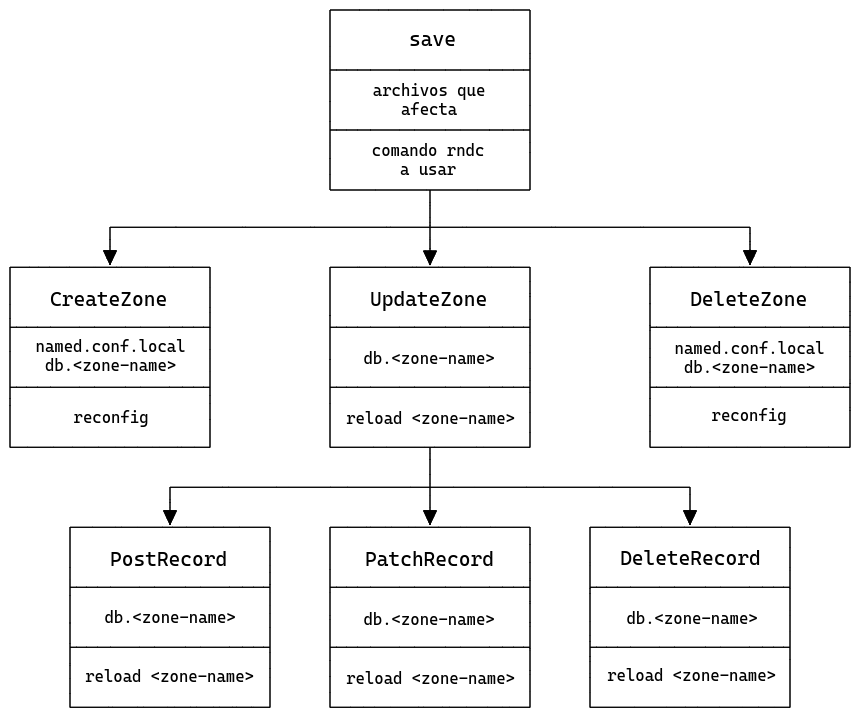
\includegraphics[width=\linewidth]{draws/split-save.png}
    \caption{Funciones que siguen el diseño de \textbf{save} para dividir la lógica.}
    \label{fig:split-save}
\end{figure}

Un cambio en la configuración por alguna de estas funcione es originado por una invocación a los puntos finales de la API. Por tanto cabe la posibilidad de que se realicen de forma concurrente en memoria. Siendo así se hace necesario limitar el acceso concurrente de escritura para evitar la corrupción de los datos haciendo uso de una instancia de \verb|sync.Mutex|. Cuando una modificación arriba a la API, la función a ser invocada toma acceso sobre este bloqueo, realiza la escritura en disco y memoria y luego lo libera.

La función principal del bloqueo es mantener la consistencia entre la información que se encuentra en memoria y en disco, asegurando que cada escritura en memoria tenga su sucesiva escritura en disco. El AST puede implementar su propio mecanismo para manejar el acceso concurrente en memoria, de igual forma se puede hacer a la hora de implementar la escritura en los archivos de configuración del disco. Pero estos dos por separado no garantizan la sincronización memoria-disco ante el acceso concurrente a la API. Además, es importante poder recuperarse de un error de escritura en disco, sin corromper la información en memoria.


Las zonas en los servidores DNS primarios son consideradas zonas de inicio de autoridad. Estas son la fuente de información para el servidor maestro y sus esclavos. Son representadas por un registro de tipo \verb|SOA| (\textit{Start Of Authority}) que contiene información administrativa y de importancia para los servidores secundarios. Los diferentes campos que contiene indican cada que tiempo los servidores secundarios deben consultar al primario por actualizaciones, cada que tiempo consultar por cambios en el número de serie y después de que intervalo detenerse los esclavos en caso de fallo en el maestro. Un aumento en el número de serie indica a los servidores secundarios que ha ocurrido una actualización en la zona y por tanto se debe iniciar una transferencia.

\begin{lstlisting}[frame=single, numbers=none, caption=Ejemplo de zona con \textit{SOA}.]
$ORIGIN example.com.
$TTL 86400
@   IN  SOA     ns.example.com. admin@example.com (
        2022110300  ;Serial
        7200        ;Refresh
        3600        ;Retry
        1209600     ;Expire
        3600        ;Negative response caching TTL
)
\end{lstlisting}

Por tanto es de vital importancia para el funcionamiento del servicio DNS que el número de serie sea incrementado en cada modificación a la zona, a pesar de que se pueda enviar una consulta de tipo \verb|NOTIFY| a los esclavos para alertar de una transferencia de zona. El número de serie es un entero positivo que indica la versión de la copia original de la zona, por lo general se puede usar como valor la fecha de cambio más dos dígitos para el caso en el que ocurran múltiples modificaciones el mismo día.

De esta forma, en la implementación, es realizada la actualización de la versión de la zona cada vez que se persisten cambios en la configuración DNS.

\begin{lstlisting}[frame=single, language=Go]
// Generates a new serial for the SOA record.
// Generated serials follows the format YYYYMMDDNN where NN is a two digits identifier.
func (dc *DomainConf) UpdateSerial() {
    now := time.Now().UTC()
    newSerial := uint(now.Year()*1_000_000 + int(now.Month())*10_000 + now.Day()*100)
    if dc.SOARecord.Serial >= newSerial {
        dc.SOARecord.Serial = dc.SOARecord.Serial + 1
    } else {
        dc.SOARecord.Serial = newSerial
    }
}
\end{lstlisting}

Según los aspectos definidos en esta sección se muestran a continuación la función \verb|CreateZone|, una de las mencionadas en la Figura \ref{fig:split-save} y que refleja el comportamiento de \verb|save| y de forma general el conjunto de funciones en que está dividida.

\label{func:create-zone}
\begin{lstlisting}[frame=single, language=Go, escapechar=|, caption=Ejemplo de la función que añade una nueva zona al servidor DNS.]
func (bm *BindService) CreateZone(data *schemas.DomainData) (*parser.DomainConf, error) {
    // Get write access to the filesystem and release it when done
    bm.Mutex.Lock()
    defer bm.Mutex.Unlock()

    // Validate that the new zone is not defined already 
    if _, ok := bm.Domains[data.Origin]; ok {
        return nil, fmt.Errorf("domain %s exists already", data.Origin)
    }

    // Create the new zone from received data
    dConf := &parser.DomainConf{
        Origin: data.Origin,
        Ttl:    data.Ttl,
        SOARecord: &parser.SOARecord{
            NameServer: data.NameServer,
            Admin:      data.Admin,
            Refresh:    data.Refresh,
            Retry:      data.Retry,
            Expire:     data.Expire,
            Minimum:    data.Minimum,
        },
        Records: []parser.Record{
            parser.NSRecord{NameServer: data.NameServer, Type: "NS"},
            parser.ARecord{Name: data.NameServer, Ip: data.NSIp, Type: "A"},
        },
    }

	bindConf := *bm.BindConf

	if err := bindConf.AddZone(dConf); err != nil {
		return nil, err
	}

    // Write new changes to BIND files and rollback on error
	rollbackDConf, err := dConf.WriteToDisk(dConf.GetFilename())
	if err != nil {
		rollbackDConf()
		return nil, err
	}

	rollbackBindConf, err := bindConf.WriteToDisk(bm.ZonesFilePath)
	if err != nil {
		rollbackDConf()
		rollbackBindConf()
		return nil, err
	}

    // Notify BIND about the new update|\label{line:call-reconf}|
	if err := bm.Reconfig(); err != nil {
		rollbackDConf()|\label{line:reconf-roll1}|
		rollbackBindConf()|\label{line:reconf-roll2}|
		return nil, err
	}

    // Sync changes on memory|\label{line:sync-mem}|
	bm.BindConf = &bindConf
	bm.Domains[dConf.Origin] = dConf

	return dConf, nil
}
\end{lstlisting}

Retomando el funcionamiento de \hyperref[proc:save]{\textbf{save}}, el método anterior primeramente toma control sobre el sistema de archivos del sistema de almacenamiento, evitando la escritura concurrente por otras invocaciones a la API. Luego verifica que la información a ser introducida en la configuración del servidor de nombres es válida usando la que se tiene de forma local en memoria. Una vez confirmado que los cambios pueden ser persistidos, pasa a efectuarse la escritura en disco, en este caso en dos archivos (\verb|/etc/bin/named.conf.local| y \verb|/var/cache/lib/db.<zone-name>|). Cuando es efectuada la escritura de la configuración, se debe notificar a BIND de los cambios, en este caso haciendo uso del comando \verb|rndc reconfig| a través de Docker, invocación realizada por \verb|Reconfig| (línea \ref{line:call-reconf}). El último estado de \verb|save| es ejecutado a partir de la línea \ref{line:sync-mem}, donde se almacenan en memoria las estructuras que validaron y aplicaron los cambios a la configuración antes de ser persistida.

\section{Manejo de errores}

Ambos parsers hacen uso de su respectivo método \verb|WriteToDisk| para llevar el AST resultante a una cadena de texto y escribirla en un archivo de texto plano. Esta función puede tener errores debido a que algún proceso externo a la API tenga bloqueado el recurso a la hora de escribir. Por tanto por conveniencia \verb|WriteToDisk| retorna una función que puede ser invocada para ``recuperar'' el sistema de archivo en caso de error y sea interrumpido el proceso de escritura.

\begin{lstlisting}[frame=single, language=Go, caption=Implementación de \textbf{WriteToDisk} para el AST de una zona.]
import (
    "fmt"
    "os"
    "strings"

    "github.com/svex99/bind-api/pkg/file"
)

// Writes the zone configuration to a plain text file.
// Returns a function that rollbacks the process.
func (dc *DomainConf) WriteToDisk(filename string) (func(), error) {
    dc.UpdateSerial()

    content := []string{
        fmt.Sprintf("$ORIGIN %s.", dc.Origin),
        fmt.Sprintf("$TTL %s", dc.Ttl),
        fmt.Sprintf(
            "@ IN SOA %s %s ( %d %d %d %d %d )",
            dc.SOARecord.NameServer, dc.SOARecord.Admin,
            dc.SOARecord.Serial, dc.SOARecord.Refresh, dc.SOARecord.Retry, dc.SOARecord.Expire, dc.SOARecord.Minimum,
        ),
    }
    for _, record := range dc.Records {
        content = append(content, record.String())
    }

    // Create a backup of config if file exists
    rollback := file.MakeBackup(filename)

    if err := os.WriteFile(filename, []byte(strings.Join(content, "\n")), 0666); err != nil {
        return rollback, err
    }

    return rollback, nil
}
\end{lstlisting}

La función usada para recuperar la copia de seguridad es almacenada en la variable \verb|rollback| y es retornada por la función para uso del contexto en que sea invocada. En la implementación del método \verb|CreateZone| (ver Código \ref{func:create-zone}), se puede comprender como esta función es invocada ante un error en procedimientos posteriores, como es la sucesiva escritura en disco o notificar al servidor de BIND sobre los cambios en la configuración.

La función \verb|MakeBackup| es la encargada de realizar la copia de seguridad de los archivos a modificar y capturar el contexto para realizar la recuperación. Dicha función se muestra a continuación.

\begin{lstlisting}[frame=single, language=Go, caption=Función encargada de mantener una copia de seguridad al modificar los archivos de BIND.]
import (
    "log"
    "os"
)

// Makes a backup (.bak file) of a plain text file
// Returns a function that rollbacks the backup file
func MakeBackup(filename string) func() {
    backup := filename + ".bak"
    bak_err := os.Rename(filename, backup)
    rollback := func() {
        if bak_err == nil {
            if err := os.Rename(backup, filename); err != nil {
                panic(err)
            }
        }
    }
    return rollback
}
\end{lstlisting}

Cuando se notifica al servidor de nombres para que actualice su servicio con los nuevos cambios es porque ya fueron modificados sus archivos de configuración. Estos cambios pueden haber sido realizados a solo un archivo de zona o adicionalmente al de configuración (ver Figura \ref{fig:split-save}). En caso de un error porque no haya comunicación con el servidor DNS o este no este en ejecución, la copia de seguridad es recuperada y la API retorna error ante el pedido. Este comportamiento también puede ser apreciado en el ejemplo de código de \verb|CreateZone| (línea \ref{line:call-reconf}), y como ante un error se recupera tanto el archivo de zona, como el de configuración (líneas \ref{line:reconf-roll1} y \ref{line:reconf-roll2} respectivamente).

\section{Despliegue de los Servicios}

\subsection{Ejecución con Compose}

- Discutir el docker-compose.yml creado.

- Interacción con los volúmenes compartidos entre la api y bind.

\subsection{Imagen para la API}

- Discutir las principales consideraciones a la hora de contenedorizar la API.

\subsection{Imagen de BIND 9}

- Consideraciones a la hora de ejecutar el servicio de bind

\section{Experimentación}

\subsection{Consumo de memoria ante el aumento de la cantidad de zonas y/o registros}

\subsection{Latencia ante el aumento de la cantidad de zonas y/o registros}
